Es ist nun naheliegend, die Menge \(\Theta_k\) mit der verbundenen Summe zu versehen. Es sind einige Lemmata notwendig, um zu zeigen, dass dies eine wohldefinierte Gruppenstruktur ergibt. 
\begin{lemma}\label{lem:simp_crit}
    Ein einfach zusammenh\"angender Kobordismus \(\mathcal{W}\) von \(\mathcal{M}\) zu \(\mathcal{N}\) ist genau dann ein H-Kobordismus, wenn \(H_*(\mathcal{W},\mathcal{M})=0\) gilt.
\end{lemma}
\begin{proof}
    Die Hinrichtung ist trivial. Seien nun \(H_*(\mathcal{W},\mathcal{M})=0\) und \(\iota\colon\mathcal{M}\hookrightarrow\mathcal{W}\) sowie \(j\colon\mathcal{N}\hookrightarrow\mathcal{W}\) die Inklusionen. Aus der Annahme folgt, dass  \(\iota\) ein Quasi-Isomorphismus ist. Dann folgt auch \(H^*(\mathcal{W},\mathcal{M})=0\) und aus der Lefschetz-Dualit\"at
    \[H_*(\mathcal{W},\mathcal{N})\cong H^{n+1-*}(\mathcal{W},\mathcal{M})=0\,,\]
    sodass auch \(j_*\) ein Quasi-Isomorphismus ist. Da \(\mathcal{W}\), \(\mathcal{M}\) und \(\mathcal{N}\) einfach zusammenh\"angend sind, folgt aus dem Satz von Whitehead, zusammen mit dem Satz von Hurewicz, dass die Inklusionen auch Homotopie\"aquivalenzen sind. 
\end{proof}
Das additive Inverse in \(\Theta_k\) ist offenbar die H-Kobordismus-Klasse der Standardsph\"are. Diese l\"asst sich wie folgt beschreiben.
\begin{lemma}\label{lem:h_cob_cont}
    Eine einfach zusammenh\"angende Mannigfaltigkeit \(\mathcal{M}^n\) ist genau dann Rand einer kontrahierbaren Mannigfaltigkeit \(\mathcal{W}^{n+1}\), wenn sie zu der Standardsph\"are H-kobordant ist.
\end{lemma}
\begin{proof}
    \subsubsection*{Hinrichtung}
        Sei \(\mathcal{M}\) Rand der kontrahierbaren Mannigfaltigkeit \(\mathcal{W}\). Sei \(\mathcal{D}\) eine eingebettete Scheibe und \({\mathcal{W}^{\prime}:=\mathcal{W}\setminus\mathring{\mathcal{D}}}\). Dann ist \(\partial\mathcal{W}^{\prime}\cong\mathcal{M}\sqcup-\mathcal{S}\) und \(\mathcal{W}^{\prime}\) ein Kobordismus. Per Ausschneidung folgt
        \[H_*(\mathcal{W}^{\prime},\partial\mathcal{D})\overcong{Aus.}H(\mathcal{W},\mathcal{D})\cong\Tilde{H}(\mathcal{W})=0\,,\]
        da \(\mathcal{W}\) einfach zusammenh\"angend ist, folgt aus Lemma \ref{lem:simp_crit}, dass \(\mathcal{W}^{\prime}\) ein H-Kobordismus ist.
        
    \subsubsection*{R\"uckrichtung}
        Sei \(\mathcal{M}\) mithilfe des Kobordismus \(\mathcal{W}^{\prime}\) zu der \(n\)-Sph\"are H-kobordant. Setze
        \[\mathcal{W}:=\mathcal{W}^{\prime}\mathop{+}^{\mathbb{S}^n}\mathbb{D}^{n+1}\,.\]
        Per Annahme gilt \(H_*(\mathcal{W}^{\prime},\mathbb{S}^n)=0\), sodass erneut
        \[H(\mathcal{W},\mathcal{D})\overcong{Aus.}H_*(\mathcal{W}^{\prime},\partial\mathcal{D})=0\]
        folgt. Da \(\mathcal{W}\) einfach zusammenh\"angend ist, ist sie zu dem kontrahierbaren Raum \(\mathcal{D}\) homotopie\"aquivalent und somit selbst kontrahierbar.
\end{proof}
\newpage
\begin{lemma}
    Das additive Inverse einer Homotopiesph\"are \(\mathcal{M}\) ist \(-\mathcal{M}\).
\end{lemma}
\begin{proof}
    W\"ahle eine Einbettung \(\Psi\colon\mathbb{R}^n+\mathbb{R}^n\hookrightarrow\mathbb{I}\times\mathbb{R}^n\) wie in Abbildung \ref{fig:sum_of_r}. F\"ur Details siehe \cite{kosinski1992differential} Kapitel VI Satz 1.3. Zu einer Verklebeabbildung \({\Phi\colon\mathbb{R}^n\hookrightarrow\mathcal{M}}\) ergibt dies eine Einbettung
    \[\im\Phi+\im\Phi\hookrightarrow\mathbb{I}\times\im\Phi\subseteq\mathbb{I}\times\mathcal{M}\,.\]
    Wird diese Einbettung \"uber \(\mathcal{M}\setminus\im\Phi\hookrightarrow0\times\mathcal{M}\) und \(-\mathcal{M}\setminus\im\Phi\hookrightarrow1\times\mathcal{M}\) zu einer Einbettung \(\mathcal{M}+(-\mathcal{M})\hookrightarrow\mathcal{M}\times\mathbb{I}\) fortgesetzt, ergibt sich eine Situation analog zu Abbildung \ref{fig:sum_of_r}. Das Bild dieser Einbettung, also auch \(\mathcal{M}+(-\mathcal{M})\), berandet eine Mannigfaltigkeit, die zu \(\mathcal{M}\), aus der eine offene Scheibe entfernt wurde, homotopie\"aquivalent ist. Diese muss jedoch kontrahierbar sein, da \(\mathcal{M}\) eine Homotopiesph\"are ist. Die Aussage folgt aus Lemma \ref{lem:h_cob_cont}.
\end{proof}

\begin{figure}
    \centering
    \begin{tikzpicture}
        \draw [pattern = north west lines]
            (-2.5, 1) -- node [above] {\(\mathbb{R}+\mathbb{R}\)} (-1.5, 1) arc (90:-90:1) -- (-2.5, -1);
        \draw [pattern = north west lines]
            (2.5, 1) -- (1.5, 1) arc (90:270:1) -- (2.5, -1)
            (-2.5, 0) edge [blue] (-0.5, 0) 
            (0.5, 0) edge [blue] (2.5, 0)
            (-3, 0) node {\(\mathbb{R}\setminus\mathring{\mathbb{D}}\)}
        ;
    \end{tikzpicture}
    \caption{Eine Einbettung \(\mathbb{R}+\mathbb{R}\hookrightarrow\mathbb{I}\times\mathbb{R}\). Ihr Bild berandet die schraffierte Mannigfaltigkeit, die die blaue Mannigfaltigkeit als Deformationsretrakt enth\"alt.}\label{fig:sum_of_r}
\end{figure}
\begin{lemma}
    Sind \(\mathcal{M}^n\) und \(\mathcal{M}^{\prime}\) geschlossen, einfach zusammenh\"angend und H-kobordant, sind es auch \(\mathcal{M}+\mathcal{N}\) und \(\mathcal{M}^{\prime}+\mathcal{N}\).
\end{lemma}
\begin{proof}
    Es kann angenommen werden, dass \(n\geq3\) ist. Sei \(\mathcal{W}_1\) ein H-Ko\-bor\-dis\-mus mit \(\partial\mathcal{W}_1=-\mathcal{M}^{\prime}\sqcup\mathcal{M}\). Da \(\mathcal{W}_1\) zu\-sam\-men\-h\"ang\-end ist, existiert eine Einbettung \(\iota\colon(\mathbb{I},\partial\,\mathbb{I})\hookrightarrow(\mathcal{W}_1,\partial\mathcal{W}_1)\) einer ordentlichen Untermannigfaltigkeit \(\mathcal{I}\), die Punkte \(p\in\mathcal{M}\) und \(p^{\prime}\in\mathcal{M}^{\prime}\) verbindet. Sei weiter \(\mathcal{W}_2:=\mathcal{N}\times\mathbb{I}\). Definiere den Kobordismus
    \[\mathcal{W}:=\mathcal{W}_1\mathop{+}^{\mathcal{I}}\mathcal{W}_2\quad\text{mit}\quad\partial\mathcal{W}\cong-\left(\mathcal{M}^{\prime}+\mathcal{N}\right)\sqcup\left(\mathcal{M}+\mathcal{N}\right)\,.\]
    Es bleibt zu zeigen, dass die Inklusionen \(\mathcal{M}+\mathcal{N}\hookrightarrow\mathcal{W}\) und \(\mathcal{M}^{\prime}+\mathcal{N}\hookrightarrow\mathcal{W}\) Homotopie\"aquivalenzen sind. Betrachte zun\"achst die Inklusion \(\iota\colon\mathcal{M}\hookrightarrow\mathcal{W}_1\). Da \(\mathcal{I}\cong\mathbb{I}\) kontrahierbar ist, ist das Normalenb\"undel in \(\mathcal{W}_1\) trivial, sodass eine Umgebung von \(\mathcal{I}\) zu \(\mathbb{I}\times\mathbb{R}^n\) diffeomorph ist. Das kommutative Diagramm
    \begin{equation}
        \begin{aligned}\label{eq:lem_sumHCob_01}
            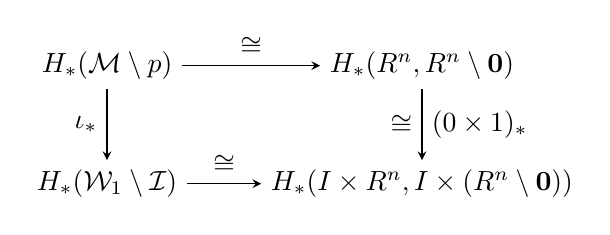
\begin{tikzpicture}
                \draw
                    (0, 0) node (A) {\(H_*(\mathcal{M}\setminus p)\)}
                    (4, 0) node (B) {\(H_*(\mathbb{R}^n,\mathbb{R}^n\setminus\mathbf{0})\)}
                    (0, -1.5) node (D) {\(H_*(\mathcal{W}_1\setminus\mathcal{I})\)}
                    (4, -1.5) node (E) {\(H_*(\mathbb{I}\times\mathbb{R}^n,\mathbb{I}\times(\mathbb{R}^n\setminus\mathbf{0}))\)}

                    (A) edge [-stealth] node [above] {\(\cong\)} (B)
                    (A) edge [-stealth] node [left] {\(\iota_*\)} (D)
                    (B) edge [-stealth] node [right] {\((0\times\mathbbm{1})_*\)} node [left] {\(\cong\)} (E)
                    (D) edge [-stealth] node [above] {\(\cong\)} (E)
                    ;
            \end{tikzpicture}
        \end{aligned}
    \end{equation}
    zeigt, dass die linke Abbildung ein Isomorphismus ist. Dann folgt aus dem F\"unfer\-lemma, dass auch die rechte Abbildung folgenden Diagrammes ein Isomorphismus sein muss.
    \begin{equation}
        \begin{aligned}\label{eq:lem_sumHCob_02}
            \begin{tikzpicture}
            \draw
                (0, 0) node (A) {\(H_*(\mathcal{M}\setminus p)\)}
                (3, 0) node (B) {\(H_*(\mathcal{M})\)}
                (6, 0) node (C) {\(H_*(\mathcal{M},\mathcal{M}\setminus p)\)}
                (0, -1.5) node (D) {\(H_*(\mathcal{W}_1\setminus\mathcal{I})\)}
                (3, -1.5) node (E) {\(H_*(\mathcal{W}_1)\)}
                (6, -1.5) node (F) {\(H_*(\mathcal{W}_1,\mathcal{W}_1\setminus\mathcal{I})\)}

                (A) edge [-stealth] (B)
                (A) edge [-stealth] node [left] {\(\cong\)} node [right] {\tiny\eqref{eq:lem_sumHCob_01}} (D)
                (B) edge [-stealth] (C)
                (B) edge [-stealth] node [left] {\(\cong\)} node [right] {\tiny H.Kob.} (E)
                (C) edge [-stealth] node [left] {\(\cong\)} node [right] {\tiny Fünferlemma} (F)
                (D) edge [-stealth] (E)
                (E) edge [-stealth] (F)
                ;
            \end{tikzpicture}
        \end{aligned}
    \end{equation}
    Betrachte nun die relative Mayer-Vietoris-Folge der Zerlegung von \((\mathcal{W},\mathcal{M}+\mathcal{N})\) durch die Bilder von \((\mathcal{W}_1\setminus\mathcal{I},\mathcal{M}\setminus p)\) und \((\mathcal{W}_2\setminus\mathbb{I},\mathcal{N}\setminus q)\). Es gilt
    \[H_*\left(\mathcal{W}_1\setminus\mathcal{I}\cap\mathcal{W}_2\setminus\mathbb{I},\mathcal{M}\setminus p\cap\mathcal{N}\setminus q\right)\cong H_*\left(\mathbb{I}\times(\mathbb{R}^n\setminus\mathbf{0}),\mathbb{R}^n\setminus\mathbf{0}\right)=0\,.\]
    Aus der Exaktheit der Mayer-Vietoris-Folge
    \[0\overeq{\eqref{eq:lem_sumHCob_02}}H_*(\mathcal{W}_1\setminus\mathcal{I},\mathcal{M}\setminus p)\oplus H_*(\mathcal{W}_2\setminus\mathbb{I},\mathcal{N}\setminus p)\to H_*(\mathcal{W},\mathcal{M}+\mathcal{N})\to0\,,\]
    folgt nun, dass auch \(H_*(\mathcal{W},\mathcal{M}+\mathcal{N})=0\) ist. Da \(\mathcal{W}\) f\"ur \(n\geq3\) weiterhin einfach zusammenh\"angend ist, folgt die Aussage aus Lemma \ref{lem:simp_crit}.
\end{proof}

\begin{lemma}
    Die verbundene Summe zweier Homotopiesph\"aren ist eine Homotopiesph\"are.
\end{lemma}
\begin{proof}
    F\"ur \(0<i<n\) gilt \(H_i(\mathcal{M}+\mathcal{N})\cong H_i(\mathcal{M})\oplus H_i(\mathcal{N})=0\), sodass \(\mathcal{M}+\mathcal{N}\) wegen
    \[H_0(\mathcal{M}+\mathcal{N})\cong H_n(\mathcal{M}+\mathcal{N})\cong\mathbb{Z}\quad\text{und}\quad H_j(\mathcal{M}+\mathcal{N})=0\quad\text{f\"ur}\quad j>n\]
    die gleichen Homologiegruppen wie die Sph\"are besitzt. Aus dem Satz von Seifert-van-Kampen folgt
    \[\pi_1(\mathcal{M}+\mathcal{N})\cong\pi_1(\mathcal{M})\times\pi_1(\mathcal{N})=0\]
    sodas \(\mathcal{M}+\mathcal{N}\) einfach zusammenh\"angend, und wegen dem Satz von Whitehead auch \((n-1)\)-zusammenh\"angend ist. Aus dem Satz von Hurewicz folgt, dass ein
    \[\eqcl{f}\in\pi_n(\mathcal{M}+\mathcal{N})\cong H_n(\mathcal{M}+\mathcal{N})\cong\mathbb{Z}\,,\]
    also eine Abbildung \(f\colon\mathbb{S}^n\to\mathcal{M}+\mathcal{N}\) des Grades eins existiert. Diese induziert in allen Dimensionen Isomorphismen \(f_*\colon H_i(\mathbb{S}^n)\to H_i(\mathcal{M}+\mathcal{N})\). Erneut folgt aus dem Satz von Whitehead, dass \(f\) eine Homotopie\"aquivalenz ist.
\end{proof}
